\chapter{Redundancy Elimination \Author{F. Chow}}
\inputprogress
\graphicspath{{img/}{pre_not_helped/img/}{part3/pre_not_helped/img/}}
\chapterauthor{F. Chow}

\section{Introduction}

Redundancy elimination is an 
important category of optimizations performed by modern optimizing compilers.
In the course of program execution, certain computations may be repeated
multiple times that yield the same results.  Such redundant
computations can be eliminated by saving the results of the non-redundant 
computations for reuse at the redundant computations.

There are two types of redundancies: \emph{full} redundancy and 
\emph{partial} redundancy.  A computation is fully redundant if the 
computation has occurred earlier regardless of the flow of control.
The elimination of full redundancy is also called common subexpression
elimination, and if applied at the global scope, it is called global common
subexpression elimination.  A computation is partially redundant if the 
computation has occurred only along certain paths.  Full redundancy can be
regarded as a special case of partial redundancy where the computation has
occurred regardless of which path is taken.

There are two different methods for deciding whether two computations are the 
same: the \emph{lexical} method and the \emph{semantic} method.  
Under the lexical method, two computations are the same if they
are written the same way using variables and/or constants before converting
to SSA, like $a+3$.  In this case, redundancy can arise only if the 
variables' values have not changed between the occurrences of the computation.
Under the semantic method, two computations are the same if they are 
the same operation performed on operands that are
not necessarily identical by name, but known to have the same values.
For example, $a+b$ and $a+c$ will compute the same result
if $b$ and $c$ are known to hold the same value.
In this chapter, we are mostly dealing with lexically identified
expressions.  Our algorithm discussion will focus on the optimization of an
expression, like $a+b$, that appears in the program.
The compiler will repeat the redundancy elimination algorithm on all the other 
lexically identified expressions in the program.
Section~\ref{section:Part3:Pre_not_helped:SemanticPRE} will discuss redundancy 
elimination among expressions that have been semantically proven to yield 
the same value.

The concept of partial redundancy was first introduced by Morel and 
Renvoise.  Before the technique of partial redundancy 
elimination was developed, optimizing compilers have been performing
global common subexpression elimination and loop invariant code motion in
separate global optimization phases.  In their seminal work \cite{MR79}, 
Morel and Renvoise showed that
global common subexpressions and loop-invariant computations are special
cases of partial redundancy that can be subsumed by the single
optimization of partial redundancy
elimination (PRE).  Morel and Renvoise formulated PRE as a code placement
problem, in which the best set of insertion points for the
expression being optimized is to be determined.  
Such insertions render some original
computations to be fully redundant, so they can be trivially
deleted.  The PRE algorithm developed by Morel and Renvoise
involves bi-directional data flow analysis, which incurs more overhead
than uni-directional data flow analysis.  In addition, their algorithm
does not yield optimal results in certain situations.

An better placement strategy, called lazy code motion (LCM), was later 
developed by Knoop {\it et al} \cite{Knoop92}\cite{Knoop94}.  It improved on
Morel and Renvoise's results by avoiding unnecessary code movements and by
removing the bi-directional nature of the original PRE data flow analysis.
The code placement produced by lazy code motion is optimal: the number of 
computations during execution time cannot
be further reduced by \emph{safe} code motion \cite{Kennedy72}, and the
lifetimes of the temporaries introduced for storing the computed values are 
minimized. After lazy code motion was introduced, there have been alternative 
formulations of PRE algorithms that achieve the same optimal results, 
but differ in the formulation approach and implementation 
details\cite{DS93}\cite{Dhamdhere02}\cite{Paleri03}\cite{XueKnoop06}.

The above approaches to PRE are all based on encoding program properties 
in bit vector forms and the iterative solution of data flow equations.
Since the bit vector representation uses basic blocks as its granularity,
a separate algorithm is needed to detect and suppress local common
subexpressions.
An SSA-based approach to solve PRE was proposed by Chow {\it et al} 
\cite{Chow97}\cite{Kennedy99}.  Their SSAPRE algorithm is an adaptation of LCM
to take advantage of the use-def information inherent in SSA.  It avoids
having to encode data flow information in bit vector form, and eliminates the
need for a separate algorithm to suppress local common subexpressionsi.
Their algorithm was first to make use of SSA to solve data flow problems
for expressions in the program, taking advantage of SSA's sparse representation
so that fewer number of steps are needed to propagate data flow information.  
The SSAPRE algorithm thus brings the many
desirable characteristics of SSA-based solution techniques to PRE, and 
further advance our understanding of this important optimization. 
Because SSAPRE operates on a sparse representation, it precludes the need
for any alternative formulation to its algorithm.

In this chapter, we only cover the conceptual bases of SSAPRE for the purpose
of getting an intuitive understanding of its inner workings.  The readers are
referred to the original publications for the full 
algorithm\cite{Chow97}\cite{Kennedy99}.

\section{Why PRE and SSA are related}
\label{section:Part3:Pre_not_helped:PRErelatedtoSSA}

Figure~\ref{fig: pre-examples} shows the two most basic forms of partial
redundancy.  In Figure~\ref{fig: pre-examples}(a), $a+b$ is redundant when 
the right path is taken.
In Figure~\ref{fig: pre-examples}(b), $a+b$ is redundant whenever the 
branch-back edge of the loop is taken.  Both are examples of \emph{strictly}
partial redundancies, in which insertions are required to eliminate the
redundancies.  In contrast, a full redundancy can be deleted without requiring 
any insertion.

\begin{figure}
\centering
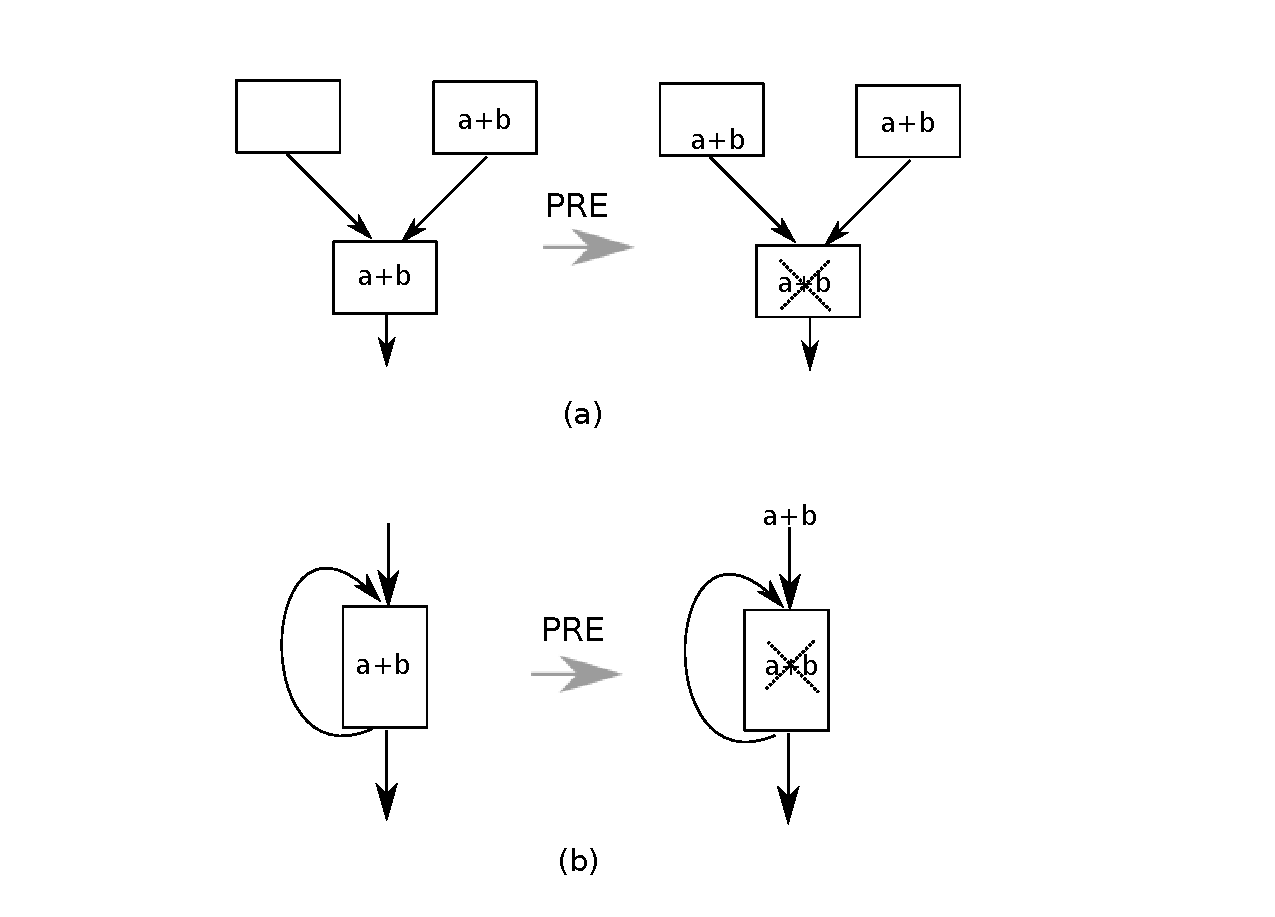
\includegraphics[scale=0.45]{fig-pre-examples.pdf}
\caption{Two basic examples of partial redundancy elimination.}
\label{fig: pre-examples}
\end{figure}

We can visualize the impact on redundancies of a single computation
as shown in Figure~\ref{fig: ssapre-motive}.  
In the region of the control flow graph dominated by the occurrence of $a+b$, 
any further occurrence of $a+b$ is fully redundant, assuming $a$ and $b$ are
not modified.  Following the program flow,
once we are past the dominance frontiers, any further occurrence of $a+b$ is
partially redundant.  In constructing SSA form, dominance frontiers are where
$\phi$'s are inserted.   Since partial redundancies start at dominance
frontiers, it must be related to SSA's $\phi$'s.  In fact, the same sparse
approach to modeling the use-def relationships among the occurrences of
a program variable can be used to model the redundancy relationships among 
the different occurrences of $a+b$.

\begin{figure}
\centering
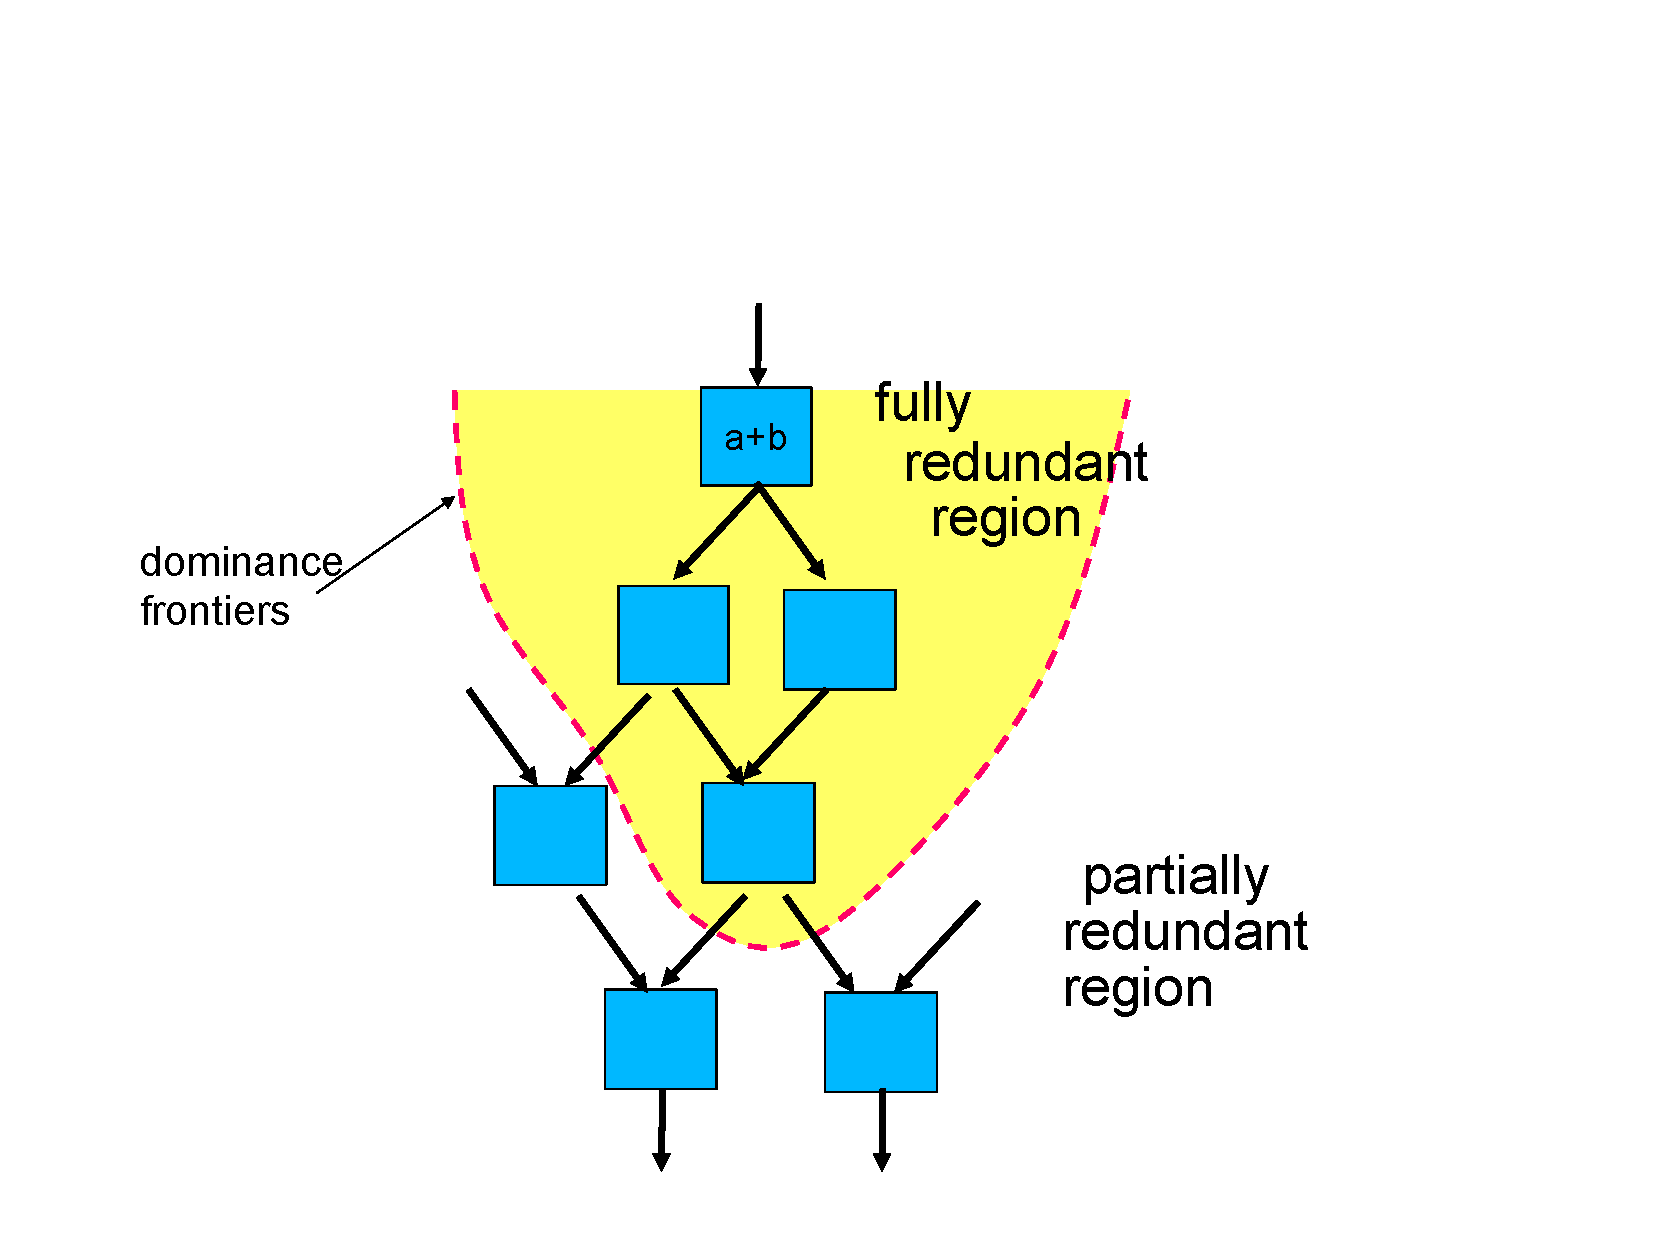
\includegraphics[scale=0.35]{fig-ssapre-motive.pdf}
\caption{Dominance frontiers are boundaries between fully and partially redundant regions.}
\label{fig: ssapre-motive}
\end{figure}

We assume the input program is already in SSA form.  If an occurrence
$a_j+b_j$ is redundant with respect to $a_i+b_i$, our representation has 
redundancy edges that connect $a_i+b_i$ to
$a_j+b_j$.  To expose potential partial redundancies, we introduce the 
operator $\Phi$ at the dominance frontiers of the occurrences, which has the 
effect of factoring the redundancy edges at merge points in the control
flow graph.\footnote{Adhering to SSAPRE's convention, we use lower case 
$\phi$'s in the SSA form of variables and upper case $\Phi$'s
in the SSA form for expressions.} The resulting \emph{factored redundancy 
graph} (FRG) can be regarded as the SSA form for expressions.

To make the expression SSA form more intuitive, we introduce the 
hypothetical temporary $h$,
which can be thought of as the temporary that will be used to store the value
of the expression for reuse in order to suppress redundant computations.
The constructed SSA form for $h$ is not precise, because we have not yet 
determined where $h$ should be defined or used.

The SSA form for $h$ is constructed in two steps similar to ordinary SSA
form: the $\Phi$-Insertion step followed by the Renaming step.  
In the $\Phi$-Insertion 
step, we insert $\Phi$'s at the dominance frontiers of all the expression 
occurrences, to ensure that we do not miss any possible placement positions
for the purpose of PRE, as in Figure~\ref{fig: phi-insertion}(a).
We also insert $\Phi$'s caused by expression alteration.
Such $\Phi$'s are triggered by the occurrence of $\phi$'s
for any of the operands in the expression.
In Figure~\ref{fig: phi-insertion}(b), the $\Phi$ at block 3 is caused by
the $\phi$ for $a$ in the same block, which in turns reflects the
assignment to $a$ in block 2.

\begin{figure}
\centering
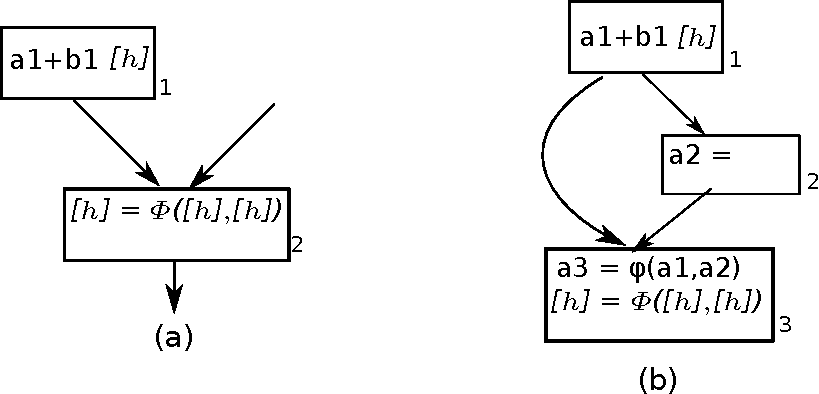
\includegraphics[scale=0.45]{fig-phi-insertion.pdf}
\caption{Examples of $\Phi$ insertion}
\label{fig: phi-insertion}
\end{figure}

The Renaming step assigns SSA versions to $h$ such that occurrences
renamed to idential $h$-versions will compute to the same values.
We conduct a pre-order traversal of the dominator tree similar to the renaming
step in SSA construction for variables, but with the following modifications.
In addition to a renaming stack for each variable, we
maintain a renaming stack for the expression. Entries on the expression
stack are popped as our dominator tree traversal backtracks past the
blocks where the expression originally received the version.  
Maintaining the variable and expression stacks
together allows us to decide efficiently whether two occurrences of an
expression should be given the same $h$-version.

There are three kinds of occurrences of the expression in the program:
(a) the occurrences in the original program, which we call \emph{real}
occurrences; (b) the $\Phi$'s inserted in the $\Phi$-Insertion step; and
(c) $\Phi$ operands, which are regarded as occurring at the ends of the
predecessor blocks of their corresponding edges.  During the visitation in 
Renaming, a $\Phi$'s is always given a new version.  For a non-$\Phi$, i.e.
cases (a) and (c),
we check the current version of every variable in the expression (the
version on the top of each variable's renaming stack) against the version of
the corresponding variable in the occurrence on the top of the expression's
renaming stack.  If all the variable versions match, we assign it the same
version as the top of the expression's renaming stack.  If any of the 
variable versions does not match, for case (a), we assign it a new version, as
in the example of Figure~\ref{fig: rename}(a); for case (c),
we assign the special class $\bot$ to the $\Phi$ operand to denote that
the value of the expression is unavailable at that point, as in the example
of Figure~\ref{fig: rename}(b).  If a new version is assigned, we push
the version on the expression stack.

\begin{figure}
\centering
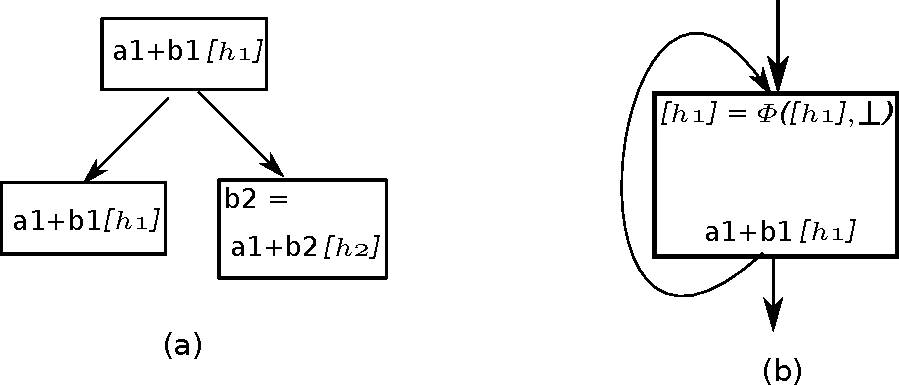
\includegraphics[scale=0.45]{fig-rename.pdf}
\caption{Examples of expression renaming}
\label{fig: rename}
\end{figure}
  
The FRG captures all the redundancies of $a+b$ in the program.  
In fact, it contains just the right
amount of information for determining the optimal code placement.  Because
strictly partial redundancies can only occur at the $\Phi$ nodes,
insertions for PRE only need to be considered at the $\Phi$'s.

\section{How SSAPRE Works}
\label{section:Part3:Pre_not_helped:SSAPRE}

Referring to the expression being optimized as $X$,
we use the term \emph{placement} to denote the set of points in the 
\emph{optimized} program where $X$'s computation occurs. In contrast,
\emph{original computation points} refer to the points in the \emph{original} 
program where $X$'s computation took place.  The objective of SSAPRE is to find
a placement that satisfies the following four criteria in this order:
\begin{enumerate}
\item Correctness --- $X$ is fully available at all the original computation
points.
\item Safety --- There is no insertion of $X$ on any path that did not 
originally contain $X$. 
\item Computational optimality ---No other safe placement can result in fewer 
computations of $X$ on any path in the program.
\item Lifetime optimality --- Subject to the computational optimality,
the life range of the temporary introduced to store $X$ is minimized.
\end{enumerate}

Each occurrence of $X$ at its original computation point can be qualified
with exactly one of the following attributes:
\begin{itemize}
\item fully redundant
\item strictly partially redundant (SPR)
\item non-redundant
\end{itemize}

As a code placement problem, SSAPRE follows the same two-step process used
in all PRE algorithsm.  The first step determines the best set of insertion 
points that render as many SPR occurrences fully redundant as possible.
The second step deletes fully redundant computations taking into account the
effects of the inserted computations.  Since the second full redundancy
elimination step is 
trivial and well understood, the challenge lies in the first step
for coming up with the best set of insertion points.  The first step will
tackle the safety, computational optimality and lifetime optimality criteria,
while the correctness criterion is delegated to the second step.
For the rest of this section, we only focus on the first step for
finding the best insertion points, which is driven by the SPR occurrences.

We assume that all \emph{critical edges}
in the control flow graph have been removed by inserting empty basic blocks
at such edges\footnote{A critical edge is one whose tail block has multiple
successors and whose head block has multiple predecessors.}\cite{Rosen88}.
In the SSAPRE approach, insertions are only performed at $\Phi$ operands.
When we say a $\Phi$ is a candidate for insertion, it means we will consider
inserting at its operands to render $X$ available at the entry to the basic
block containing that $\Phi$.  An insertion at a $\Phi$ operand means inserting
$X$ at the incoming edge corresponding to that $\Phi$ operand.  In reality,
the actual insertion is done at the end of the predecessor block.

\subsection{The Safety Criterion}

As we have pointed out at the end of 
Section~\ref{section:Part3:Pre_not_helped:PRErelatedtoSSA},
insertions only need to be considered at the $\Phi$'s.
The safety criterion implies that we can only insert at $\Phi$'s where $X$ 
is \emph{downsafe} (fully anticipated).  Thus, we perform data flow analysis on
the FRG to determine the \emph{downsafe} attribute for $\Phi$'s.
Data flow analysis can be performed with linear complexity on SSA graphs, which
we illustrate with the Downsafety computation.

A $\Phi$ is not \emph{downsafe} if there is a control flow path from that 
$\Phi$ along which the expression is not evaluated before program exit or 
before 
being altered by redefinition of one of its variables.  Except for loops with
no exit, this can happen only due to one of the following cases: (a) there
is a path to exit or an alteration of the expression
along which the $\Phi$ result version is not used; or (b) the $\Phi$ result
version appears as the operand of another $\Phi$ that is not \emph{downsafe}.
Case (a) represents the initialization for our backward propagation of 
$\neg downsafe$; all other $\Phi$'s are initially marked $downsafe$.
The Downsafety propagation is based on case (b).  Since a real occurrence of 
the expression blocks the case (b) propagation, we mark each
$\Phi$ operand with a flag \emph{has\_real\_use} when the path to the $\Phi$
operand crosses a real occurrence of the same version of $X$ to effect the
blocking.  Figure~\ref{fig: downsafety} gives the DownSafety propagation 
algorithm.

\begin{figure}[!ht]
{\bf procedure} Reset\_downsafe($X$) 
\{
\begin{code}
\x1 {\bf if} ($has\_real\_use(X)$ {\bf or} $def(X)$ is not a $\Phi$)
\x2   {\bf return}
\x1 $f \leftarrow def(X)$
\x1 {\bf if} ({\bf not} $downsafe(f)$)
\x2   {\bf return}
\x1 $downsafe(f) \leftarrow$ false
\x1 {\bf for} each operand $\omega$ of $f$ {\bf do}
\x2   Reset\_downsafe($\omega$)
\end{code}
\}

{\bf procedure} DownSafety
\{
\begin{code}
\x1 {\bf for} each $f \in$ \{$\Phi$'s in the program\} {\bf do}
\x2   {\bf if} ({\bf not} $downsafe(f)$)
\x3     {\bf for} each operand $\omega$ of $f$ {\bf do}
\x4	  Reset\_downsafe($\omega$)
\end{code}
\}
\caption{Algorithm for DownSafety}
\label{fig: downsafety}
\end{figure}

\subsection{The Computational Optimality Criterion}

The best set of $\Phi$'s for performing insertion is arrived at via a
process of elimination.  At this point, we have
eliminated the unsafe $\Phi$'s based on the safety criterion.  
We now seek to disqualify more $\Phi$'s from
insertion consideration by identifying those that we can prove as
violating the computational optimality criterion.  This is done
by performing the CanBeAvail propagation, which is in the forward direction.

The CanBeAvail propagation is derived from the well-understood full 
availability analysis.
We define a $\Phi$ \emph{can\_be\_avail} if and only if inserting there will 
not violate computational optimality.  In other words, a $\Phi$ is 
$\neg can\_be\_avail$ if and only if inserting there violates computational
optimality.  
This can happen only due to one of the following cases: (a) 
the $\Phi$ is not \emph{downsafe} and one of its operands is $\bot$; or (b)
the $\Phi$ is not \emph{downsafe} and it has an operand that is a 
$\neg can\_be\_avail \Phi$ and that operand is not \emph{has\_real\_use}.
Case (a) represents the initialization for our forward propagation of
$\neg can\_be\_avail$; all other $\Phi$'s are initially marked
\emph{can\_be\_avail}.  The CanBeAvail propagation is based on case (b).

After \emph{can\_be\_avail} has been computed, it is possible to perform 
insertions at
all the \emph{can\_be\_avail} $\Phi$'s.  There would be full redundancies
created among the insertions themselves, but they would not affect 
computational optimality because the subsequent full redundancy elimination 
step will remove any fully redundant inserted or non-inserted computation, 
leaving the earliest computations as the optimal code 
placement.\footnote{This outcome is referred to as \emph{busy code motion} 
by Knoop {\it et al.} to contrast with their lazy code motion.}

\subsection{The Lifetime Optimality Criterion}

To fulfill lifetime optimality, we perform a second forward propagation called
Later that is derived from the well-understood partial availability 
analysis.  The purpose is to disqualify \emph{can\_be\_avail} $\Phi$'s that are
partially available based on the original occurrences of $X$.
A $\Phi$ is marked \emph{later} if it is not necessary to insert there because
a later insertion is possible.  We optimistically regard all the
\emph{can\_be\_avail} $\Phi$'s to be \emph{later}, except the following cases:
(a) the $\Phi$ has an operand defined by a real computation; or (b) the $\Phi$
has an operand that is a $\Phi$ marked not \emph{later}.  Case (a) represents
the initialization for our forward propgation of not \emph{later}; all other
\emph{can\_be\_avail} $\Phi$'s are marked \emph{later}.  The Later
propagation is based on case (b).

\begin{figure}
\centering
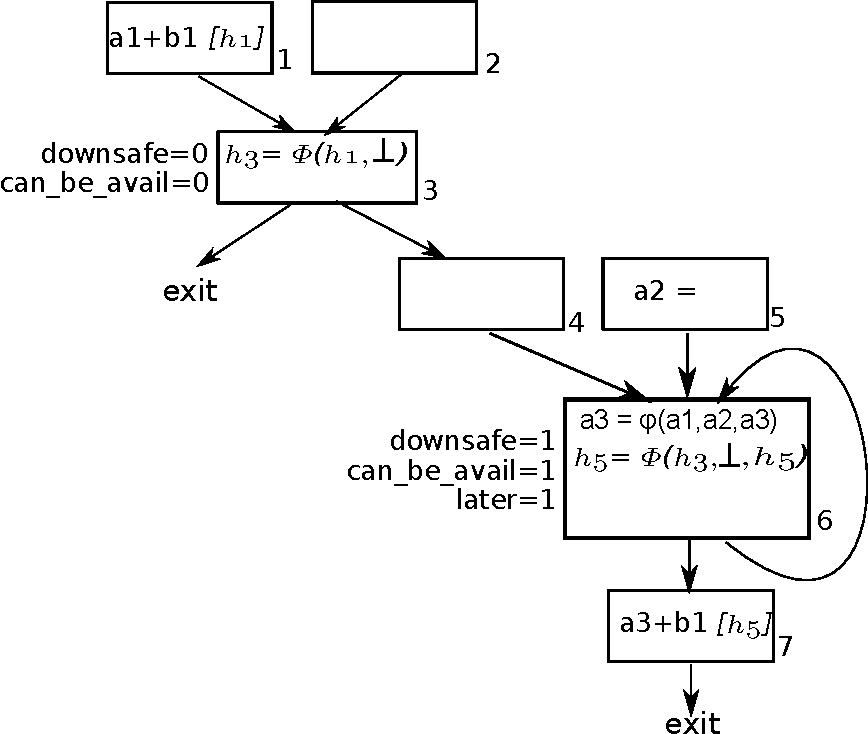
\includegraphics[scale=0.45]{fig-later-example.pdf}
\caption{Example to show the need of the \emph{Later} attribute}
\label{fig: later-example}
\end{figure}

The final $\Phi$'s for performing insertion are the $\Phi$'s where 
\emph{can\_be\_avail} and $\neg later$ hold.  We call such $\Phi$'s
\emph{will\_be\_avail}.  At each of these $\Phi$'s,
insertion is performed at each operand that satisfies either of the following
condition:
\begin{enumerate}
\item it is $\bot$; or
\item \emph{has\_real\_use} is false and it is defined by a 
$\neg will\_be\_avail \Phi$.
\end{enumerate}

We illustrate our discussion in this section with the example of 
Figure~\ref{fig: later-example}, where the program exhibits partial redundancy
that cannot be removed by safe code motion.  The two $\Phi$'s with their 
computed data flow attributes are as shown.  If insertions were based on
\emph{can\_be\_avail}, $a+b$ would have been inserted at blocks 4 and 5,
which would have resulted in unnecessary code motion that increases
register pressure.  By considering \emph{later}, no insertion is performed,
which is optimal under safe PRE for this example.
 
\section{Speculative PRE}

If we ignore the safety requirement of PRE discussed in 
Section~\ref{section:Part3:Pre_not_helped:SSAPRE}, the resulting code motion
will involve speculation.
In the absence of systems support, speculation should only be applied to
expressions that will not cause runtime exceptions or faults, since such
exceptions or faults will alter the external behavior of the program.  
For example, indirect loads from unknown pointer values cannot be speculated
unless the systems would mask out the effect of loading from invalid addresses.
Speculative code motion suppresses
redundancy in some path at the expense of another path where the computation 
is added but result is unused.  As long as the paths that are burdened with
more computations are executed less frequently than the paths where the
redundant computations are avoided, a net gain in program performance can be
achieved.  Thus, speculative code motion should only be performed when there
are clues about the relative execution frequencies of the paths involved.

Without profile data, speculative PRE can be conservatively performed by
restricting it to loop-invariant computations.  
Figure~\ref{fig: spec-pre} shows
a loop-invariant computation $a+b$ that occurs in a branch inside the loop.
This loop-invariant code motion is speculative because, depending on the
branch condition inside the loop, it may be executed zero time, while moving it
to the loop header causes it to execute one time. This speculative 
loop-invariant code motion is profitable unless the path inside the loop
containing the expression is never taken, which is usually not the case.
When performing SSAPRE, marking $\Phi$'s located at the start of loop bodies
downsafe will effect speculative loop invariant code motion\cite{Lo98}. 

\begin{figure}
\centering
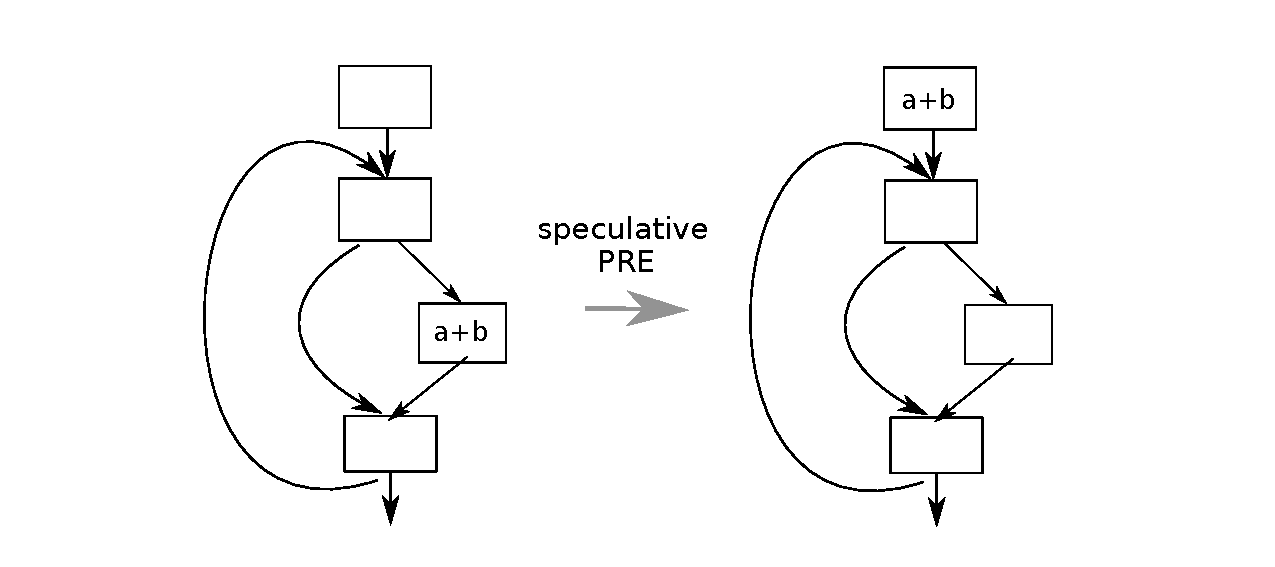
\includegraphics[scale=0.55]{fig-spec-pre.pdf}
\caption{Speculative loop-invariant code motion}
\label{fig: spec-pre}
\end{figure}

To enable more code motion of unsafe operations, Murphy {\it et al.} modify 
SSAPRE to use the \emph{fault-safety} property\cite{Murphy08}.   
They define \emph{dangerous}
computations as operations that may fault but will otherwise have no observable
side effects.  Such computations include indirect loads and divides.  Such
dangerous computations are sometimes protected by tests (or guards) placed in
the code by the programmers.  Compilers for languages like Java also insert 
runtime checks to ensure faults never occur. When such a test occurs in the
program, the dangerous computation is said to be \emph{safety-dependent} on
the control flow point that establishes its safety.  A dangerous instruction
is \emph{fault-safe} at any point in the program where its safety dependence
is satisfied.

Murphy {\it et al.} represent safety dependences as value dependences in the
form of the abstract \emph{tau values} described in \cite{Menon06}.  Each check
that succeeds will define a tau value on its fall-through path.  During SSAPRE,
dangerous computations will have additional \emph{tau} operands attached to 
them.  The tau
operands are also variables in SSA form, so their definitions can
be found by following the use-def edges.  The compiler inserts the definitions
of the taus also with abstract right-hand-side values, like {\bf tauedge}.
Because they are abstract, they
are omitted in the generated code after the SSAPRE phase.  A dangerous
computation can be defined to have more than one tau operands, depending on
its semantics.  When all its tau operands have definitions, 
it means the computation is fault-safe; otherwise, it is unsafe.  
By including the tau operands into consideration, speculative PRE automatically
honors the fault-safety of dangerous computations when it performs speculative
code motion.

As an example, if we replace the expression $a+b$ in Figure~\ref{fig: spec-pre}
by $a/b$, the speculative code motion cannot be performed because if $b$ is 0,
the speculative insertion of $a/b$ at the loop header will cause a run-time
divide-by-zero fault.  In Figure~\ref{fig: spec-div}, the program contains a 
non-zero test for $b$.  We define a tau operand for $a/b$ in SSAPRE to
provide the information whether a non-zero test for b is available.  The
presense of the non-zero test for $b$ causes the compiler to insert the
definition of $tau1$ with the abstract right-hand-side value {\bf tauedge}.
Since the divide inside the loop $a_1/b_1,tau_1$ has a tau operand whose
definition is visible, speculative SSAPRE will force the $\Phi$ at the head
of the loop body to be downsafe.  When $a_1/b_1,tau_1$ is hoisted out of the
loop, it automatically stops at the definition of $tau_1$ because PRE obeys
value dependence.

\begin{figure}
\centering
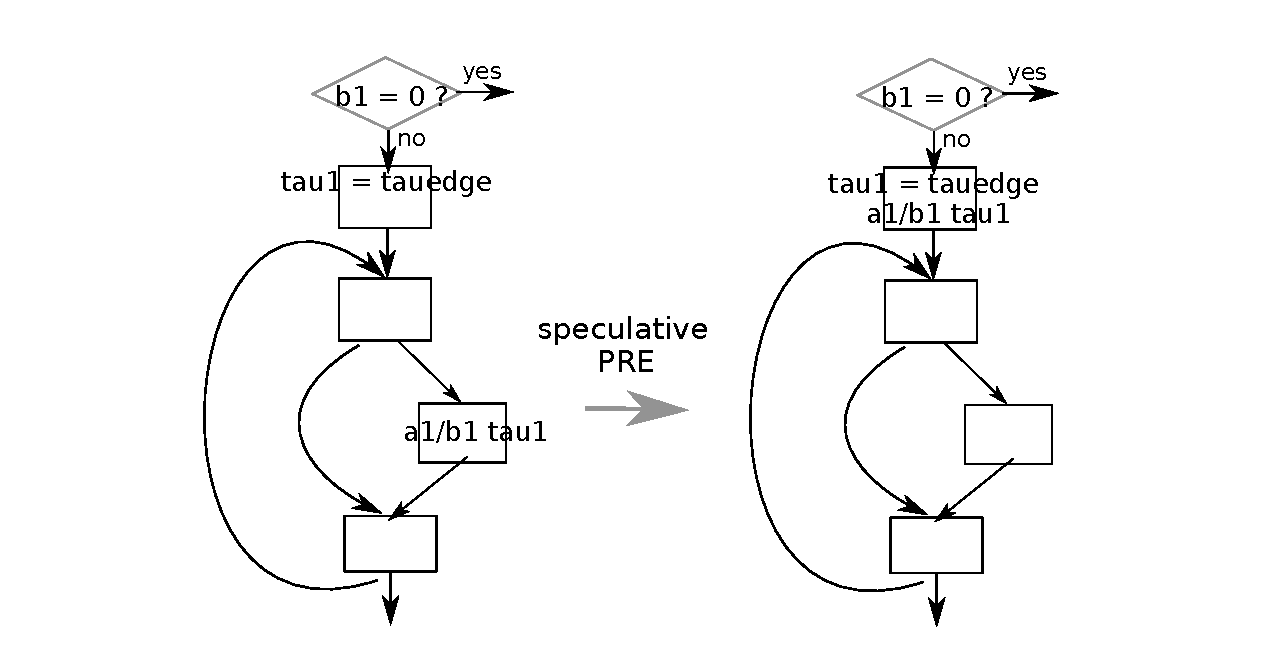
\includegraphics[scale=0.55]{fig-spec-div.pdf}
\caption{Speculative and fault-safe loop-invariant code motion}
\label{fig: spec-div}
\end{figure}

When execution profile data are available, it is possible to tailor the use
of speculation to maximize run-time performance for the execution 
that matches the profile.  Xue and Cai presented a computationally 
and lifetime optimal algorithm
for speculative PRE based on profile data\cite{Xue06}.  Their algorithm
uses bit-vector-based data flow analysis and applies minimum cut to flow
networks formed out of the control flow graph to find the optimal code
placement.  Zhou {et al.} applies the 
minimum cut approach to flow networks formed out of the FRG in the SSAPRE 
framework to achieve the same computational and lifetime optimal code 
motion\cite{zhou11}.  They showed their sparse approach based on SSA results
in smaller flow networks, enabling the optimal code placements to be 
computed more efficiently.

\section{Register Promotion via PRE}

Register promotion refers to the important task in an optimizing compiler
of identifying the data items that are candidates for register allocation 
in the program.  To represent register allocation candidates, compilers
commonly use an unlimited number of \emph{pseudo-registers}.  Pseudo-registers
are also called symbolic registers or virtual registers, to distinguish them
from real or physical registers.  Pseudo-registers have no alias, and the
process of assigning them to real registers involves only renaming them.

\subsection{Register Promotion as Placement Optimization}

Under PRE, the temporaries generated to hold the values of redundant 
computations are pseudo-registers.  Local variables determined by the compiler
to have no alias can be trivially renamed to pseudo-registers.   All remaining
register allocation candidates have to be assigned pseudo-registers through 
the process of register promotion.  Register promotion is also responsible
for generating the most efficient code to set up the data objects in
pseudo-registers.  Targets for register promotion include scalar variables,
indirectly accessd memory locations and program constants.  
Load operations are needed to put them into pseudo-registers before
they are used\footnote{Depending on the ISA, some constants may not need to be
put in registers, and they should be excluded from register promotion.}, and
when there is an assignment, a store operation is needed.  Since the goal of
register promotion is to obtain the most efficient placements for the loads and
stores, register promotion can be modeled as two separate problems: PRE of 
loads, followed by PRE of stores.

From the point of view of redundancy, loads are like expressions because the
later occurrences are the ones to be deleted.  For stores, the reverse is true:
the earlier stores are the ones to be deleted, as is evident in the examples
of Figure~\ref{fig: load-store-dual}(a) and (b).  The PRE of stores,
also called \emph{partial dead code elimination}, can thus be treated as the
dual of the PRE of loads.  Performing PRE of stores thus has the effects
of moving stores forward while inserting them as early as possible.  
Combining the effects of the PRE of loads and stores results in optimal
placements of loads and stores while minimizing the live ranges of the
pseudo-registers, by virtue of the computational and lifetime optimalities
of our PRE algorithm.

\begin{figure}
\centering
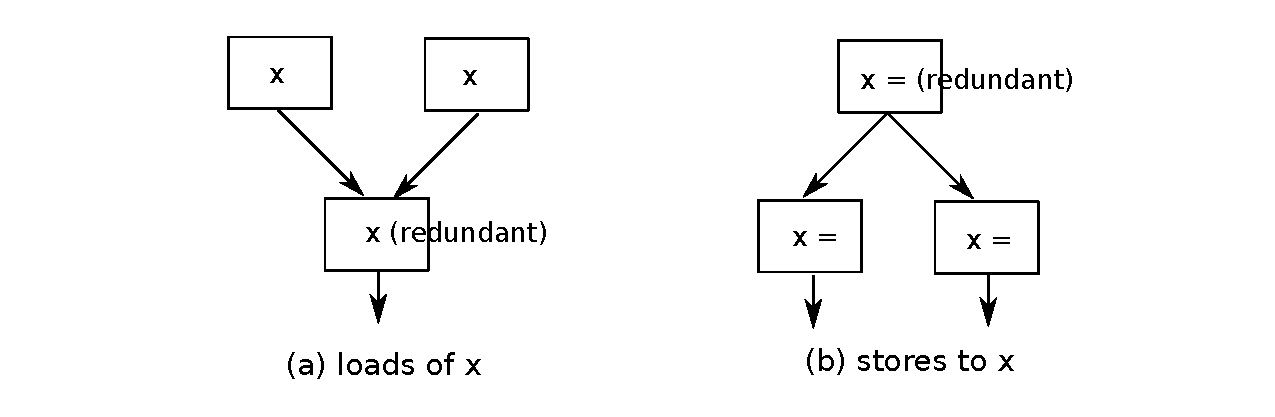
\includegraphics[scale=0.55]{fig-load-store-dual.pdf}
\caption{Duality between load and store redundancies}
\label{fig: load-store-dual}
\end{figure}

\subsection{Load Placement Optimization}

PRE applies to any computation including loads from memory locations and
loads of constants.  In program representations, loads can either be indirect 
through a pointer or direct.  Direct loads  and constants are leaves
in expression trees.  
When we apply SSAPRE to direct loads, since the hypothetical temporary $h$ can
be regarded as the candidate variable itself, the $\Phi$-insertion step and
Rename step can be streamlined.  In other words, the $\Phi$'s are the variable's
$\phi$'s, and the $h$-versions are the variable's SSA version.

When working on the PRE of memory loads, it is important to also take into
account the stores, which we call \emph{l-value} occurrences.  A store of the 
form $x \leftarrow \texttt{<expr>}$ can be regarded as being made up of the
sequence:
\begin{tabbing}
XX:\= while \= while \= while \= while \= while \= \kill

\> \> $r \leftarrow \texttt{<expr>}$ \\
\> \> $x \leftarrow r$ \\
\end{tabbing}
Because the pseudo-register $r$ contains the current value of $x$, any
subsequent occurrences of the load of $x$ can reuse the value from $r$, and
thus can be regarded as redundant.   Figure~\ref{fig: lval-occur} gives examples
of loads made redundant by stores.

\begin{figure}
\centering
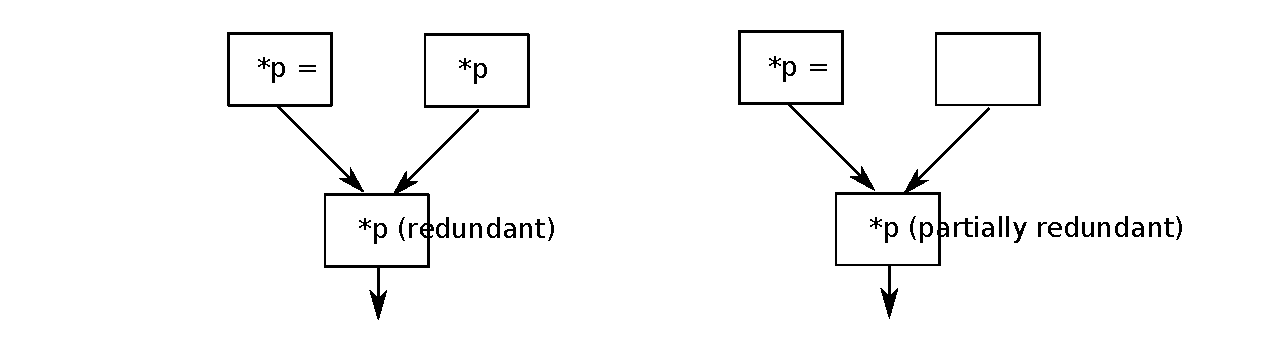
\includegraphics[scale=0.55]{fig-lval-occur}
\caption{Redundant loads after stores}
\label{fig: lval-occur}
\end{figure}

When we perform the PRE of loads, we thus include the l-value occurrences into
consideration.  The $\Phi$-insertion step will insert $\Phi$'s at the iterated
dominance frontiers of l-value occurrences.  In the Rename step, an l-value
occurrence is always given a new $h$-version, because a store is a definition.
Any subsequent load renamed to the same $h$-version is redundant with respect
to the store.

We apply the PRE of loads
first, followed by the PRE of stores.  This ordering is based on the fact that
the PRE of loads is not affected by the results of the PRE of stores, but the
PRE of loads creates more opportunities for the PRE of stores by deleting
loads that would otherwise have blocked the movement of stores.  In addition,
speculation is required for the PRE of loads and stores in order for register
promotion to do a decent job in loops.  

The example in Figure~\ref{fig: promotion-example} illustrates what we discuss
in this section.  During the PRE of loads (LPRE), $a =$ is regarded as an
l-value occurrence.  The hoisting of the load of $a$ to the loop header does
not involve speculation. The occurrence of $a =$ causes $r$ to be updated
by splitting the store into the two statements $r =$ followed by $a = r$.  In 
the PRE of stores (SPRE), speculation is needed to sink $a =$ to outside the
loop because the store occurs in a branch inside the loop.  Without performing 
LPRE first, the load of $a$ inside the loop would
have blocked the sinking of $a =$.

\begin{figure}
\centering
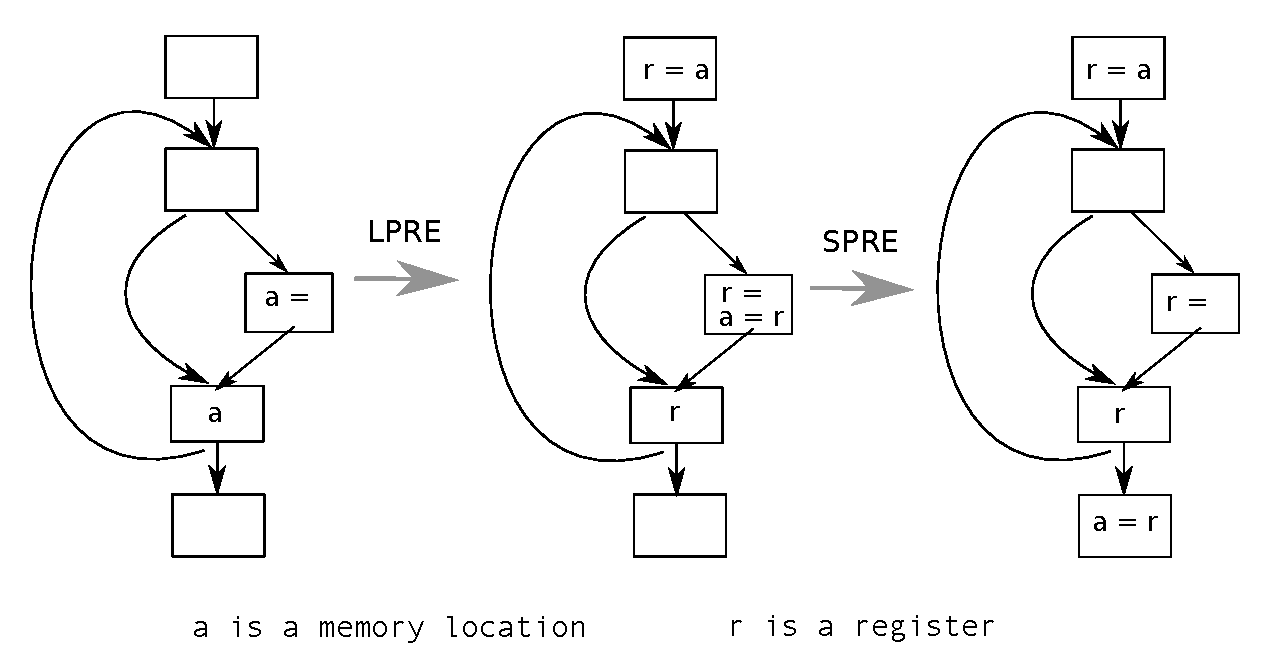
\includegraphics[scale=0.55]{fig-promotion-example.pdf}
\caption{Register promotion via load PRE followed by store PRE}
\label{fig: promotion-example}
\end{figure}

\subsection{Store Placement Optimization}

As mentioned earlier, SPRE is the dual of LPRE.
In the presence of store redundancies, the earlier occurrences are redundant.
Code motion in SPRE will have the effect of moving stores forward with respect 
to the control flow graph.  Any presence of (aliased) loads have the effect of
blocking the movement of stores or rendering the earlier stores non-redundant.

To apply the dual of the SSAPRE algorithm, it is necessary to compute a program
representation that is the dual of the SSA form, and we call this the 
\emph{static single use} form.  In SSU, use-def edges are factored at
divergence points in the control flow graph.  We call this factoring operator
$\Lambda$.  Each use of a variable establishes a new version (we say the load 
\emph{uses} the version), and every store reaches exactly one load.   The
$\Lambda$ is regarded as a use of a new version of the variable.  The use
post-dominates all the stores of its version.  The left-hand-side of the
$\Lambda$ is the multiple definitions, each of which is post-dominated by their
single uses.

We call our store PRE algorithm SSUPRE, which is made up of the corresponding 
steps in SSAPRE.   $\Lambda$-Insertion and
SSU-Rename, construct the SSU form for the variable whose store is being 
optimized.  The data flow analyses consist of UpSafety to compute the
\emph{upsafe} (fully available) attribute, CanBeAnt to compute the
\emph{can\_be\_ant} attribute and Earlier to compute the \emph{earlier}
attribute.  Though store elimination itself does not require
the introduction of temporaries, lifetime optimality still needs to be
considered for the temporaries introduced in the LPRE phase which hold the 
values to the point where the stores are placed.  It is desirable not 
to sink the stores too far down.  

\begin{figure}
\centering
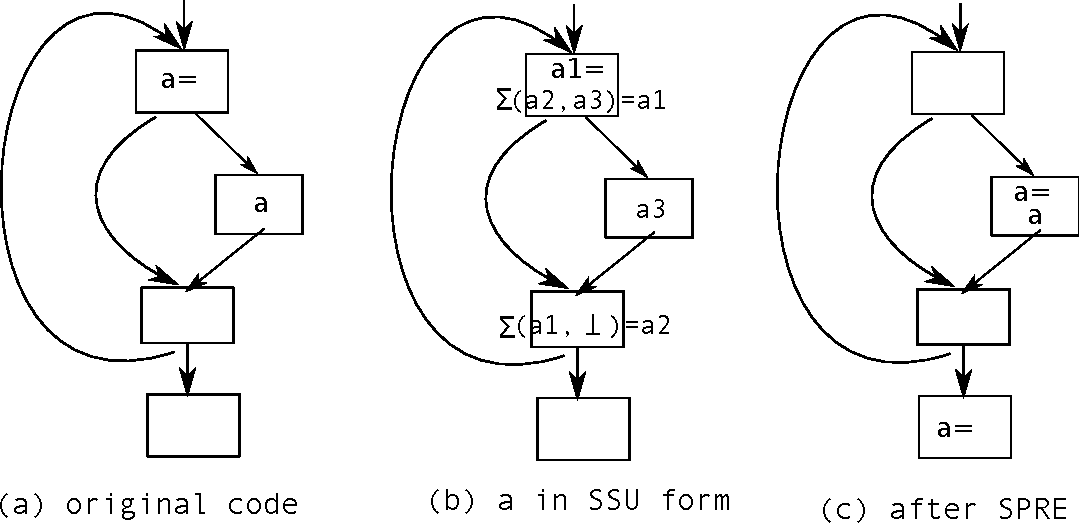
\includegraphics[scale=0.55]{fig-ssupre.pdf}
\caption{Example of program in SSU form and the result of applying SSUPRE}
\label{fig: ssupre}
\end{figure}

Figure~\ref{fig: ssupre} gives an example program with (b) being the SSU 
representation for the program in (a).  
(c) shows the result of applying SSUPRE to the code.
The store can be sunk to outside the loop only if it is also inserted in
the branch inside the loop that contains the load.  The optimized code no
longer exhibits any store redundancy.

A limitation of the above SSUPRE algorithm is that it does not apply to 
indirect stores.  It may be possible to extend the algorithm to make it
work on indirect stores as well.

\section{Redundancy via the Semantic Approach}
\label{section:Part3:Pre_not_helped:SemanticPRE}

The redundant computations stored into a temporary introduced by PRE may
be of different values because the same lexically identified expression may
yield different results at different points in the program.
Since PRE applies only to lexically identified expressions, it is not capable
of recognizing redundant computations among lexically different expressions
based on their semantics.  On the other hand, under the semantic approach, 
redundant computations can be recognized among computations that are 
semantically determined to yield the same values.

\subsection{Value Numbering}

Computations are determined to yield the same value using \emph{value numbering}
analysis techniques.  The term \emph{value number} originated from the 
hash-based method developed by Cocke and Schwartz for recognizing when two
expressions evaluate to the same value within a basic block \cite{CS70}.  
The value number of an expression tree can be regarded as the index of its
hashed entry in the hash table.  
An expression tree is hashed bottom up starting with the leaf nodes.  
Each internal node is hashed based on its operator and the value numbers of 
its operands.  Two expressions with the same
value number \emph{must} evaluate to the same value at run-time.

When the program has been put into SSA form, value number can be extended to the
global scope by assigning a unique value number to each variable version by
virtue of the single definition property \cite{Rosen88}.  Additional 
refinements to hash-based global value numbering algorithms have been proposed
by Briggs {\it et al} \cite{Briggs97}.

\begin{figure}[t]
\begin{center}
\fbox{ \parbox[t]{6.0in} {
\begin{tabbing}
XX:\= op \= op \= op \= op \= op \= \kill
Place all values computed by the same opcode in the same congruence class\\
$worklist \leftarrow$ set of all congruence classes\\
{\bf while} $worklist \neq \phi$ \\
\> Select and delete an arbitrary congruence class $c$ from $worklist$\\
\> {\bf for} each operand position $p$ of a use of $x \in c$\\
\>  \> $touched \leftarrow \phi$\\
\>  \> {\bf for} each $x \in c$\\
\>  \>  \> Add any expression in the program that uses $x$ in position $p$ to $touched$\\
\>  \> {\bf for} each class $s$ such that $\phi \subset (s \cap touched) \subset s$\\
\>  \>  \> Create a new class $n \leftarrow s \cap tourhed$\\
\>  \>  \> $s \leftarrow s - n$\\
\>  \>  \> {\bf if} $s \in worklist$ \\
\>  \>  \>  \> Add $n$ to $worklist$ \\
\>  \>  \> {\bf else}\\
\>  \>  \>  \> Add smaller of $n$ and $s$ to $worklist$\\
\end{tabbing}}}
\caption{The partitioning algorithm}
\label{fig: partition-alg}
\end{center}
\end{figure}

A second approach for determining whether two expressions compute the
same value that uses the partitioning method instead of hashing. 
First developed by
Alpern {\it et al.} \cite{AWZ88}, the algorithe partitions all the expressions
in the program into congruence classes.  Values in the same congruence class 
are considered as evaluating to identical values.  The algorithm is 
optimistic because when it starts,
it puts all expressions based on the same operator into the same
congruence class.  Given two expressions within the same congruence class, if 
their operands at the same operand position belong to different congruence
classes, the two expressions may compute to different values, and thus should
not be in the same congruence class.  This is used as the subdivision 
criterion.  As the algorithm iterates, the congruence classes are subdivided
into smaller ones while the total number of congruence classes increases.
The algorithm terminates when no more subdivision can occur.
At this point, an enumeration of the resulting congruence classes can be
used as value numbers.  The detailed algorithm is shown in 
Figure~\ref{fig: partition-alg}. In the last {\bf for} loop, 
$\phi \subset (s \cap touched) \subset s$ is the criterion for subdividing
class $s$ because the other members of $s$ that do not have $x$ at
operand position $p$ potentially compute to a different value.  
After the partition into $n$ and the new $s$,
if $s$ is not in the worklist (i.e. processed already), the 
partitioning was already stable with respect to the old $s$, and
we can add either $n$ or the new $s$ to the worklist to re-stabilize with
respect to that split of $s$.  Choosing the smaller one results in less
overhead.

Briggs {\it et al.} have also proposed additional refinements to the 
partitioning technique \cite{Briggs97}.  
Partition-based algorithms do not supercede, but 
instead complement the hash-based algorithms.
The most powerful value numbering algorithms are in fact based on
a combination of the two approaches.

\subsection{Redundancy Elimination via Value Numbering}

So far, we have only talked about finding computations that compute the
same value, but have not addressed how to use the results of such analysis 
to optimize the program.  Two computations that compute the same value do
not exhibit redundancy if they are not situated on the same
execution path.  Thus, it is logical to consider performing PRE separately
for each value number.  

If we consider the temporary $t$ that will be introduced to store the redundant
computations under value-number-based PRE, we can see that its value will
stay the same throughout its lifetime.  If there are $\phi$'s introduced for
the temporary, they will be merging identical values, and we know from
experience that such $\phi$'s are rare.  A subset of such $\phi$'s is expected 
to come from PRE's insertions, and that implies that insertions
introduced by value-number-based PRE are also rare.

Value-number-based PRE also has to deal with the additional issue of \emph{how}
to generate an insertion.  Because the same value can come from different forms
of expressions at different points in the program, it is necessary to determine
which form to use at an insertion point.  If the insertion point is outside 
the live range of any variable version that can compute that value, then the
insertion point has to be disqualified.  Due to this complexity, and the
expectation that strictly partial redundancy is rare among computations
that yield the same value, we focus only on eliminating full redundancies
among computations that have the same value number\footnote{This assumes
PRE for lexically identified expressions have been applied, which would have
removed the redundancies among lexically identified expressions that also
have the same value number.}.

Since full redundancy elimination (FRE) is a subset of PRE, we can adapt the
SSAPRE algorithm to work on value-number-identified expressions and remove
full redundancies among them.  We call this adapted algorithm VNFRE.

In VNFRE, the $\Phi$-Insertion step only needs to consider the iterated
dominance frontiers.  It is not necessary to consider the variable operands,
because as long as the value number is the same, we do not have to consider
when any variable operand's value is changed. The Renaming step is also simpler
because we also ignore the variable operands.  In fact, the only situations 
where new $h$-versions are introduced are at program entry (when the renaming 
stack is empty) and when encountering $\Phi$'s.  With the FRG constructed,
we perform the full availability analysis on the $\Phi$'s to identify
the expressions that can be deleted.

In practice, with copy propagation, constant folding and SSAPRE having been 
performed earlier, there are not much optimization opportunities left 
for VNFRE to cater to.  One useful application of VNFRE is in induction
variable collescing.  Code like the following, with multiple induction
variables, could be the result of
earlier optimizations like strength reduction:
{\tt
\begin{verbatim}
        i = 0;
        j = 0;
        while <cond> {
          i = i + 4;
          j = j + 4;
        }
\end{verbatim}
}

Value numbering will determine that at different points in the code, {\tt i}
and {\tt j} always have the same value number.  Performing VNFRE will yield the
net effect of getting rid of the extra induction variables.

\section{Conclusion}

The close relationsihp between PRE and SSA arises because 
partial redundancies can be exposed by factoring at control flow merge points.
The SSAPRE algorithm capitalizes on prior techniques developed for computing 
and manipulating SSA form.  The SSAPRE framework also shows that the 
concept and techniques of SSA can be made to apply to any program constructs, 
not just variables.  The constructed SSA graphs can then be used to 
efficiently perform sparse data flow propagation.

There are additional optimizations that can be implemented using the SSAPRE
framework that we have not covered.  They include code hoisting, register 
shrink-wrap\-ping \cite{Chow88} and live range shrinking.  Moreover, PRE has 
traditionally provided the context for integrating additional optimizations 
into its framework.  They include operator strength reduction \cite{Knoop93} 
and linear function test replacement \cite{Kennedy98}.  As a result, PRE 
has become the most powerful and encompassing optimization framework in modern 
optimizing compilers.
